%% Parity-violating experiment

An important and complementary indirect probe of new TeV-scale dynamics in flavor-conserving processes involves
ultra-precise measurements of weak neutral current amplitudes in fixed target experiments. 
In order to match the sensitivity of future collider
searches and other indirect probes, it is necessary to be able to measure amplitudes with an uncertainty
approaching $10^{-3}\times G_F$. The technique of parity-violating electron scattering, in which one measures
the fractional difference $A_{PV}$ in the cross-section for longitudinally polarized electrons scattering off 
unpolarized  targets, has attained the sensitivity to make important contributions to a comprehensive search for new 
TeV-scale dynamics in the flavor-conserving sector~\cite{ref:cl:kkannualreview}. 

A comprehensive discussion of leptonic and semi-leptonic weak neutral current processes, their respective 
sensitivitiies, and complementarity are discussed in Sec. XX of the Working Group on Nuclei and Atoms. 
In the following, we focus on one important, purely-leptonic such measurement, namely 
$A_{PV}$ in electron-electron (M\o ller) scattering.  
The SLAC E158 experiment made the first ever measurement of this observable~\cite{ref:cl:Anthony:2005pm}, 
and set
important complementary limits on contact interactions with a sensitivity comparable to the highest energy
colliders that were then running in parallel i.e. LEP-II and the Tevatron. 

Recently, the MOLLER experiment has been proposed at Jefferson Laboratory to improve on the E158
measurement by more than a factor of 5, taking advantage of the energy upgrade of the high intensity
polarized electron beam to 11 GeV~\cite{ref:cl:Dudek:2012vr}. The goal is a measurement of $A_{PV}$ to a fractional accuracy
of 2.3\%. 
The electron beam energy, luminosity and stability at Jefferson Laboratory are uniquely suited to carry out such a measurement. 
The compelling opportunity that this initiative represents can be summarized in three inter-related bullets:
\begin{enumerate}
\item New neutral current interactions are best parameterized model-independently at low energies by effective 
four-fermion interactions via the quantity $\Lambda/g$, where $g$ characterizes the strength and $\Lambda$ is the
scale of the new dynamics. The proposed $A_{PV}$ measurement is sensitive to new interaction amplitudes as 
small as $1.5\times 10^{-3}\cdot G_F$, which corresponds to a sensitivity of $\Lambda/g =  7.5$~TeV. This would be {\it the} most sensitive probe of new flavor and CP-conserving 
neutral current interactions in the leptonic sector until the advent of new lepton collider or a neutrino factory. 
\item Within the Standard Model, precision measurements of weak neutral current amplitudes can be interpreted as measurements of the weak mixing angle $\sin^2\theta_W$. The two most precise such determinations of 
$\sin^2\theta_W$ differ from each other by more than 3 standard deviations. 
While the world average is consistent with other electroweak measurements and the mass of the scalar resonance 
discovered at the LHC, choosing one or the other central value ruins this consistency and would imply very
different kinds of new high-energy dynamics. The proposed $A_{PV}$ measurement, which aims to achieve
$\delta(\sin^2\theta_W) = \pm 0.00029$, may be the only realistic way to achieve the same level of precision and interpretability in accelerator facilities that are operational over the next decade.
\item An important feature of the proposed measurement is that it would be carried out at $Q^2\ll M_Z^2$, in contrast
to the two best measurements mentioned above, which emerged from analyses of real $Z^0$ decays. A 
convenient way to parametrize a class of new physics effects, to which $Z^0$ resonance observables are 
insensitive, is via the parameter 
$X(Q^2)\equiv\alpha^{-1}(\sin^2\theta_W(Q^2)-\sin^2\theta_W(M_Z^2)$. The projected MOLLER sensitivity is 
$\delta(X)\approx 0.035$. This is by far the most sensitive reach among similar potential
measurements under discussion and probes a very interesting region of discovery space of new low
energy flavor-conserving effective amplitudes that might be induced for example by "dark'' photons with 
a tiny admixture of the Standard Model $Z^0$ boson~\cite{ref:cl:darkz}. 
\end{enumerate}

$A_{PV}$ in M\o ller scattering measures the weak charge of the electron
$Q^e_W$, which is proportional to the product of the electron's vector and axial-vector couplings to the $Z^0$ boson. 
The electroweak theory prediction at tree level in terms of the weak mixing angle is $Q^e_W = 1 - 4\sin^2\theta_W$; 
this is modified at the 1-loop level~\cite{ref:cl:Czarnecki:1995fw, ref:cl:Czarnecki:2000ic, ref:cl:Erler:2004in} and
becomes dependent on the energy scale at which the measurement is carried out, {\em i.e.} $\sin^2\theta_W$
``runs". At low energy, $Q^e_W$  is predicted to be 
$0.0469\pm 0.0006$, a $\sim 40$\%\ change of its tree level value of $\sim 0.075$ (when evaluated at $M_Z$).

The prediction for $A_{PV}$ for the proposed experimental design is 
$\approx 35$~parts per billion (ppb) and our goal is to measure this quantity with a statistical precision of 0.73 ppb
and thus achieve a 2.3\%\ measurement of $Q^e_W$. The reduction in the numerical value of $Q^e_W$ 
due to radiative corrections leads to increased fractional accuracy in the determination of the weak mixing
 angle, $\sim 0.1$\%, comparable to the two best such determinations from measurements of asymmetries in
$Z^0$ decays in the $\mathrm{e}^+\mathrm{e}^-$ colliders LEP and SLC. 

Figure.~\ref{fig:cl:s2tw} shows
the four best measurements from studies of $Z^{0}$ decays~\cite{ref:cl:lepewwg}
as well as the projected uncertainty of the MOLLER proposal. Also shown
is the Standard Model prediction for a Higgs mass ($m_H$) of 126 GeV. It can be seen that the grand average of the
four measurements is consistent with the theoretical expectation. However, the scatter in the measurements
is disconcerting; it would be very useful to have new measurements such as MOLLER with comparable precision. 
Indeed, it is going to be very difficult to achieve this sensitivity with any other method 
until the advent of new facilities, which are more than a decade away.

An additional important feature of the proposed measurement is that it will be carried out at $Q^2\ll M_Z^2$.
The two best measurements of the weak mixing angle at lower energies are those extracted from the
aforementioned SLAC E158 measurement~\cite{ref:cl:Anthony:2005pm}, 
and the measurement of the weak charge of $^{133}$Cs~\cite{ref:cl:csapv} via studies of table-top atomic parity violation. The interpretation of the latter measurement in terms of an extraction of the weak mixing angle has
been recently updated~\cite{ref:cl:cuspidate}. Figure~\ref{fig:cl:s2twvsmh} shows the dependence 
of $\sin^2\theta_W$ to $m_H$ and the two best high energy and low energy measurements discussed above.
Also shown is the projected error for the MOLLER proposal. Remarkably, many different versions of new dynamics
at the TeV scale can have a significant impact on low $Q^2$ measurements while having little impact on
$Z^0$ decay measurements because interference effects on resonance are suppressed. It can be seen that there
is still plenty of room for new physics effects to be discovered at low energy given the proposed $A_{PV}$ 
uncertainty. 

\begin{figure}[ht]
\begin{minipage}[b]{0.48\linewidth}
\centering
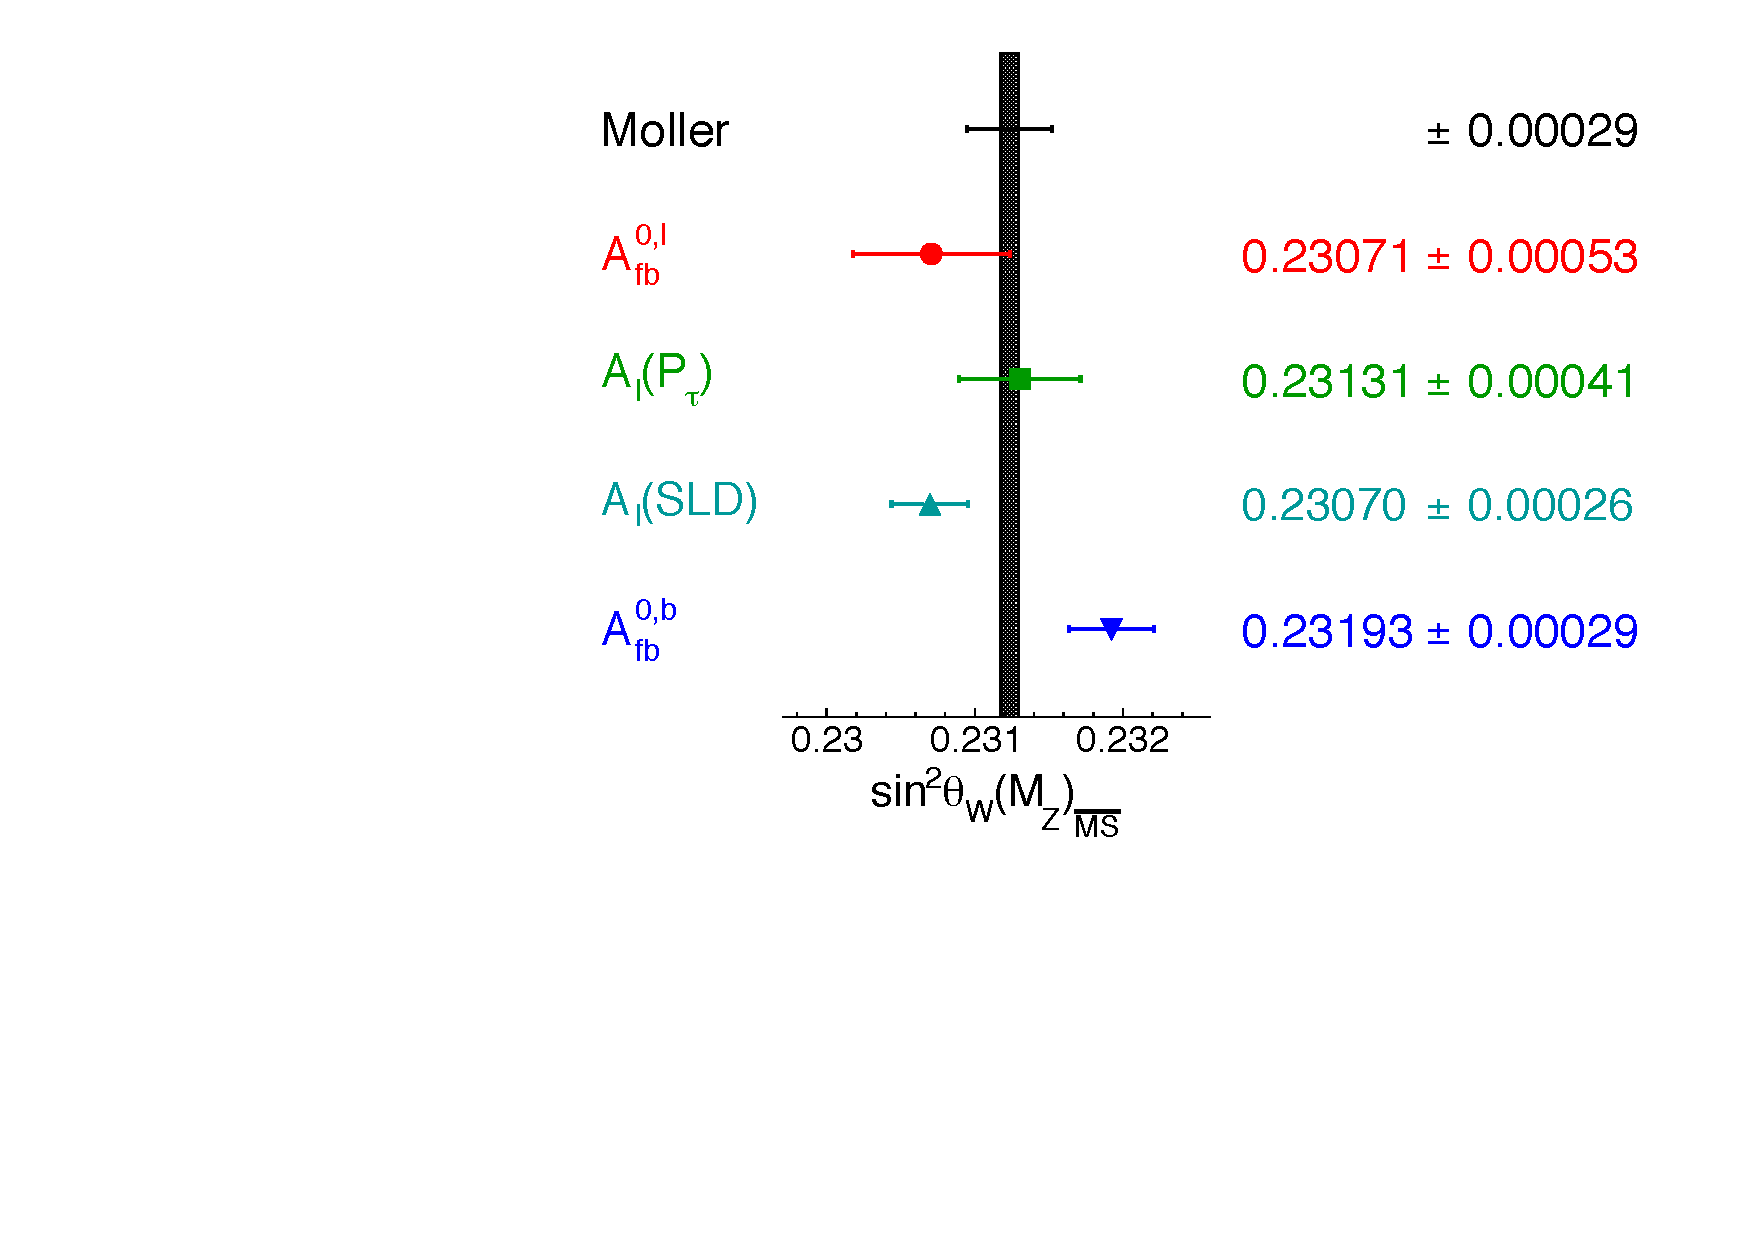
\includegraphics[width=0.95\linewidth]{ChargedLeptons/Figures/sin2thW_wmoll.pdf}
%  \includegraphics[width=0.8\linewidth]{rpv_loop_ab.eps}
  \caption{{\it The four best $\sin^2\theta_W$ measurements and the projected error of the MOLLER proposal.
  The black band represents the theoretical prediction for $m_H = 126$ GeV.}}
\label{fig:cl:s2tw}
\end{minipage}
\hspace{0.3cm}
\begin{minipage}[b]{0.48\linewidth}
\centering
    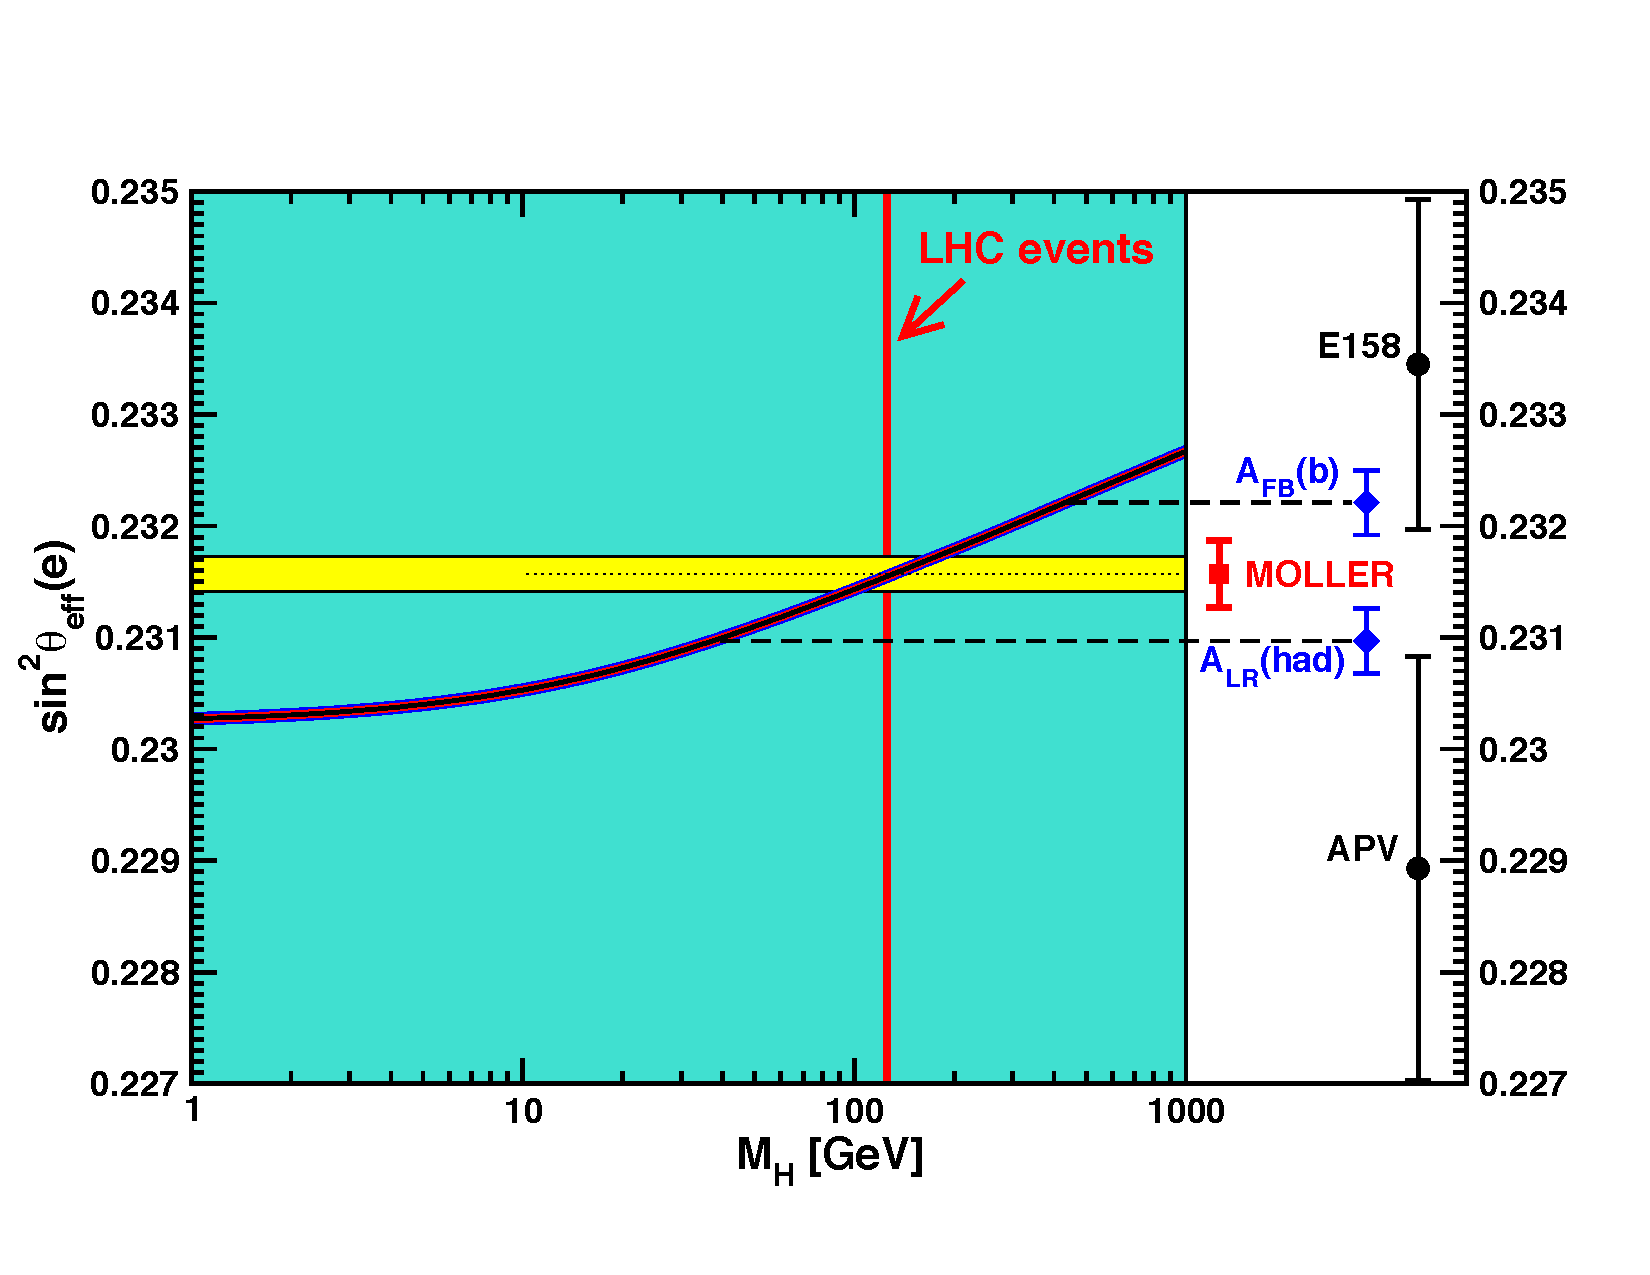
\includegraphics[width=3in]{ChargedLeptons/Figures/st2wvsmh.pdf}
  \caption{{\it $\sin^2\theta_W$ vs $m_H$. The yellow band shows the world average. The blue data points
  represent the two best high energy determinations while the black points are the most precise low energy
  determinations. The projected MOLLER error is shown in red. }}
  \label{fig:cl:s2twvsmh}
\end{minipage}
\end{figure}

At the level of sensitivity probed, the proposed measurement could be influenced by radiative loop effects of new 
particles predicted by the Minimal Supersymmetric Standard Model (MSSM). The impact on the weak charges of the
electron and the proton $Q_W^{e,p}$ have been analyzed in detail~\cite{ref:cl:Kurylov:2003zh}. A combined analysis of 
precision low energy measurements of both charged and neutral current processes can be found in a comprehensive review~\cite{ref:cl:RamseyMusolf:2006vr}, which has been recently updated~\cite{ref:cl:Erler:2013xha}. 
Inspecting a random scan over a set of MSSM parameters whose values are consistent with current precision 
measurements as well as the most recent LHC search limits from 7 and 8 TeV running, $A_{PV}$ would see 
in the effects in the range of 2 and 3 $\sigma$ at larger values of the MSSM parameter $\tan\beta$ (the ratio of vacuum expectation values of the model's two Higgs scalars) or if one of the superpartner 
masses is relatively light. 
If the assumption of R-parity conservation is relaxed (RPV), tree-level interactions could generate even deviations 
in $A_{PV}$ of opposite sign and similar magnitude. Thus, if nature is supersymmetric, the proposed measurement
would shed light on an important followup question regarding the validity of R-parity symmetry.

A comprehensive analysis of the MOLLER sensitivity to 
TeV-scale $Z^\prime$s has been carried out~\cite{ref:cl:Erler:2011iw} 
for a fairly large class of family-universal models
contained in the $E_6$ gauge group.  While models with full $E_6$ unification are already
excluded by existing precision electroweak data, the Z' bosons in these models with the same electroweak charges to SM particles are still motivated because 
they also arise in many superstring models as well as from a bottom-up approach~\cite{ref:cl:Erler:2000wu}. 
$A_{PV}$ probes
 $M_{Z^\prime} $ of order 2.5 TeV, comparable to the anticipated reach of 
early LHC running after the energy ramp-up to 13 TeV. The reach of $A_{PV}$ would be further 
enhanced in comparison 
to direct searches if one relaxes the model-dependent assumption of GUT coupling strength; indirect 
deviations scale linearly with other values of the coupling strength whereas dilepton production at colliders
has a much milder dependence on this parameter. 


%\section{Experimental Design}
The measurement would be carried out in Hall A at Jefferson Laboratory, where a 11 GeV longitudinally polarized electron beam would be incident on a 1.5 m liquid hydrogen target. M\o ller electrons (beam electrons scattering off target electrons) in the full range of the azimuth and spanning the polar angular range 5 mrad $<\theta_{lab}<$ 17 mrad, would be separated from background and brought to a ring focus $\sim 30$~m downstream of the target by a spectrometer system consisting of a pair of toroidal magnet assemblies and precision collimators. 
The M\o ller ring would be intercepted by a system of quartz detectors; the resulting Cherenkov light would provide a relative measure of the scattered flux. The experimental techniques for producing an ultra-stable polarized electron beam, systematic
control at the part per billion level, calibration techniques to control normalization errors including the degree of electron 
beam polarization at the 1\%\ level have been continuously improved over fifteen years of development at JLab.
%\section{Systematic Control}

%\section{Current Status|}
The 2007 NSAC long range plan report  comprehensively described the opportunities presented by new sensitive indirect probes such as MOLLER, and how they fit into the subfield of Fundamental Symmetries.
One of the overarching questions that serves to define this subfield is: ``What are the unseen forces that were present at the dawn of the universe but disappeared from view as the universe evolved?". To address this question and as part of the third principal recommendation, significant new investments, including MOLLER, were advocated.

MOLLER received the highest rating from the JLab Program Advisory Committee (PAC) in January 2009.
Subsequently in January 2010, 
JLab management organized a Director's review of the experiment chaired by Charles Prescott. The committee
gave strong endorsement to the experiment and encouraged the collaboration and the laboratory to develop
a full proposal to obtain construction funding.  In January 2011, 
the PAC allocated MOLLER's full beamtime request of 344 PAC days. 
More recently, the 2012 NSAC subpanel on the implementation of the Long Range Panel (the Tribble 
 Subcommittee) strongly endorsed the MOLLER project as part of the suite of investments advocated for 
 the subfield of Fundamental Symmetries.
JLab submitted a Major Item of Equipment (MIE) proposal
to DoE on behalf of the MOLLER collaboration ($\sim 100$ physicists from 30 institutions).
The goal is to obtain construction funding by 2015, with 
the hope of installing the apparatus and commissioning the experiment in 2017/18. 


